\documentclass{article}
\usepackage{polski}
\usepackage[utf8]{inputenc}
\usepackage{amsmath}
\usepackage{mathtools}
\usepackage{graphicx}
\usepackage{placeins}
\usepackage[final]{pdfpages}
\graphicspath{{Obrazki/Etap2/}}

\title{Technika automatyzacji procesów\\ Projekt - etap 2}
\author{Rafał Goluch \\ Łukasz Meyer\\ Arkadiusz Piórkowski}

\begin{document}
%\pagenumbering{gobble}

\includepdf[pages=-]{TAP_3_etap1.pdf}

\maketitle

\section{Uproszczenie transmitancji}
W pierwszej części projektu uzyskano model w postaci transmitancji:
\[
G(s)^T = \left[
\arraycolsep=5pt\def\arraystretch{1.5}
\begin{array}{cc}
\frac{0.002}{s+0.005094}\cdot e^{-230s} & \frac{0.004487s+2.286\cdot 10^{-5}}{s^2+0.01528s+5.19\cdot 10^{-5}}\cdot e^{-500} \\
0 & \frac{0.002145}{s+0.01019}\cdot e^{-270s} \\
\frac{0.002}{s+0.005094} & \frac{-0.001733s-8.826\cdot 10^{-6}}{s^2+0.01528s+5.19\cdot 10^{-5}}\cdot e^{-270} \\
0 & \frac{0.006434}{s+0.01019}\cdot e^{-270s} \\
\frac{0.002}{s+0.005094} & \frac{0.000948+4.832\cdot 10^{-6}}{s^2+0.01528s+5.19\cdot 10^{-5}}\cdot e^{-270} \\
0 & \frac{0.001609}{s+0.01019}\cdot e^{-270s}
\end{array}
\right]
\]
Człony z transmitancjami drugiego rzędu można uprościć poprzez zapisanie mianownika w formie iloczynowej, skraca się on z licznikiem (skraca się stabilny składnik - inercja pierwszego rzędu). Uzyskujemy wtedy:
\[
G(s)^T = \left[
\arraycolsep=5pt\def\arraystretch{1.5}
\begin{array}{cc}
\frac{0.3926}{196.3s+1}\cdot e^{-230s} & \frac{2.23}{100s+1}\cdot e^{-500} \\
0 & \frac{0.21}{98,1s+1}\cdot e^{-270s} \\
\frac{0.3926}{196.3s+1} & \frac{-0.173}{100s+1}\cdot e^{-270} \\
0 & \frac{0.63}{98.1s+1}\cdot e^{-270s} \\
\frac{0.3926}{196.3s+1} & \frac{10.5}{100s+1}\cdot e^{-270} \\
0 & \frac{0.16}{98.1s+1}\cdot e^{-270s}
\end{array}
\right].
\]

\newpage
\section{Analiza RGA}
Kolejnym krokiem było wyznaczenie macierzy RGA w celu określenia struktury regulacji, to znaczy przyporządkowania wielkości sterowanych $F_{Hin}$ oraz $F_C$ do wyjść $h$ oraz $T_{out}$.
Konieczne jest określenie macierzy transmitancji tylko dla wejść sterowanych (pominięcie wejść niesterowanych $T_H, T_C, F_D, T_D$).
\[
G_{RGA}(s) = \left[
\arraycolsep=5pt\def\arraystretch{1.5}
\begin{array}{cc}
\frac{0.3926}{196.3s+1}\cdot e^{-230s} & \frac{2.23}{100s+1}\cdot e^{-500} \\
\frac{0.3926}{196.3s+1} & \frac{-0.173}{100s+1}\cdot e^{-270} \\
\end{array}
\right]
\]
Macierz wzmocnień statycznych $K$:
\[
K = \left[
\begin{array}{cc}
0.3926 & 0.3926\\
2.23 & -0.173
\end{array}
\right].
\]
Natomiast macierz $\bar{K}$:
\[
\bar{K} = (K^{-1})^T = \left[
\begin{array}{cc}
-0.1834 & 2.364\\
-0.4161 & -0.4161
\end{array}
\right].
\]
Zgodnie z~\cite{regulacja_wielopetlowa} mamy wzór na względne wzmocnienie w torze $u_j \rightarrow y_i$:
\[
\lambda_{ij} = k_{ij} \cdot \bar{k_{ij}},
\]
co po obliczeniu wartości daje macierz RGA:
\[
\Lambda = \left[
\begin{array}{cc}
-0.072 & 1.072\\
0.928 & 0.072
\end{array}
\right].
\]
Na diagonali rozpoczynającej się w górnym lewym rogu macierzy uzyskano niekorzystne wartości współczynników $\lambda$, to znaczy wartości nie są bliskie 1, a także jedna z komórek ma ujemną wartość. Na drugiej diagonali uzyskano natomiast korzystne wartości, zbliżone do 1.

Powyższe oznacza, że przyporządkowanie wielkości sterowanych do wielkości regulowanych powinno być następujące:
\[
F_{Hin} \rightarrow T_{out}
\]
\[
F_C \rightarrow h
\]
Takie przyporządkowanie sprawia, że w pętli regulacji temperatury występuje bardzo duże opóźnienie (łącznie 500 sekund), jednak uznano, że istotniejsze jest spełnienie warunku o nieujemności wartości komórek macierzy RGA.

\section{Struktura regulacji}
Utworzony schemat regulacji w Simulinku przedstawiono na rysunku~\ref{fig::pid_schemat}. Zawiera on już człony odsprzęgające, opisane w rozdziale~\ref{sec::czlony_odsprzegajace}. Układ pozwala na włączenie i wyłączenie transmitancji skrośnych oraz odsprzęgających z poziomu Matlaba.

Układ posiada także bloki obcinające sygnały sterujące $F_C$ i $F_H$ (\textit{Saturation} i \textit{Saturation1}), które mogą być deaktywowane z poziomu Matlaba. Bloki te obcinają sygnał względem punktu pracy, przyjęto że może się mieścić on w zakresie $-60\frac{cm^3}{s}$ do $40\frac{cm^3}{s}$ w przypadku $\Delta F_C$ (w ten sposób sygnał $F_C$ zmienia się w zakresie od $0\frac{cm^3}{s}$ do $100\frac{cm^2}{s}$. Dla $\Delta F_H$ zakres wynosi od $-20\frac{cm^3}{s}$ do $80\frac{cm^3}{s}$, więc dopuszczalna wartość $F_H$ zmienia się od $0\frac{cm^3}{s}$ do $100\frac{cm^3}{s}$.
\begin{figure}[!htb]
	\centering
	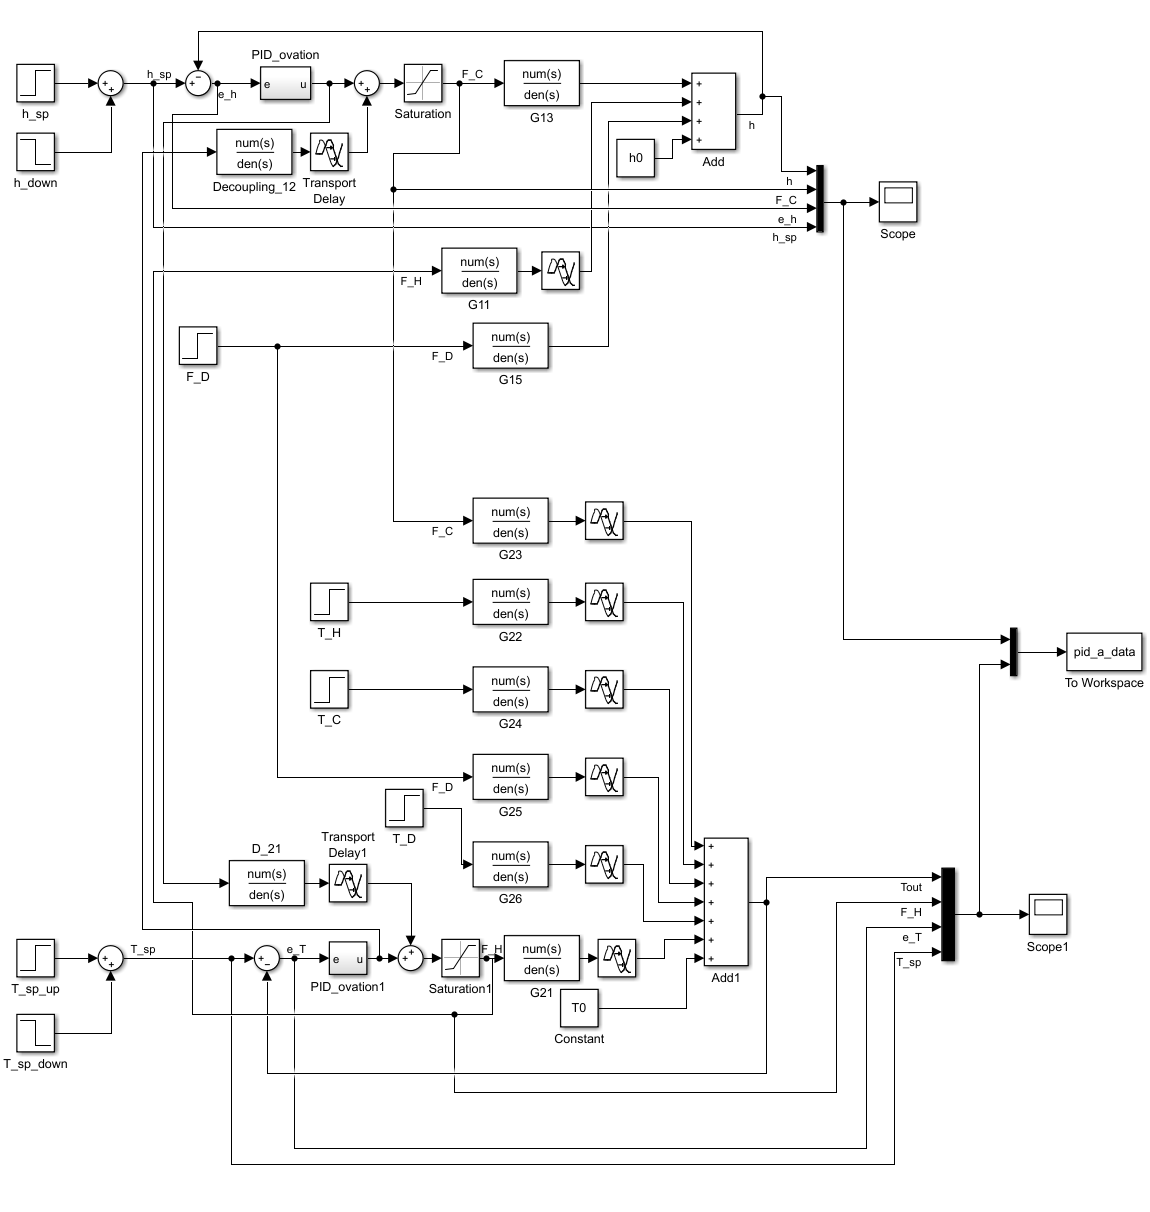
\includegraphics[width=1.1\textwidth]{pid_schemat.PNG}
	\caption{Schemat regulacji wysokości i temperatury}
	\label{fig::pid_schemat}
\end{figure}

\newpage
\section{Człony odsprzęgające}
\label{sec::czlony_odsprzegajace}
W układzie regulacji dodano bloki odsprzęgające:
\begin{itemize}
	\item $D_{12}(s)$ - transmitancja odsprzęga wpływ zmian sygnału $F_H$ na wyjście $h$
	\item $D_{21}(s)$ - transmitancja odsprzęga wpływ zmian sygnału $F_C$ na wyjście $T$
\end{itemize}
W przypadku analizowanego układu transmitancje te mają postać:
\[
D_{12}(s) = -\frac{G_{11}(s)}{G_{13}(s)} = -\frac{\frac{0.3926}{196.3s+1}\cdot e^{-230s}}{\frac{0.3926}{196.3s+1}} =  -e^{-230s}
\]
\[
\widetilde{D_{21}}(s) = -\frac{G_{23}(s)}{G_{21}(s)} = -\frac{\frac{-0.173}{100s+1}\cdot e^{-270}}{\frac{2.23}{100s+1}\cdot e^{-500}} = 0.0776\cdot e^{230s}
\]
Transmitancja $D_{12}(s)$ jest realizowalna, więc uzyskamy pełne odsprzęganie na wyjściu $h$. Transmitancja $D_{21}(s)$ zawiera blok przyspieszający $e^{230s}$, co oznacza, że nie jest realizowalna. W związku z tym transmitancję tę sprowadzono do postaci realizowalnej:
\[
D_{21}(s) = 0.0776
\]
\begin{figure}[!htb]
	\centering
	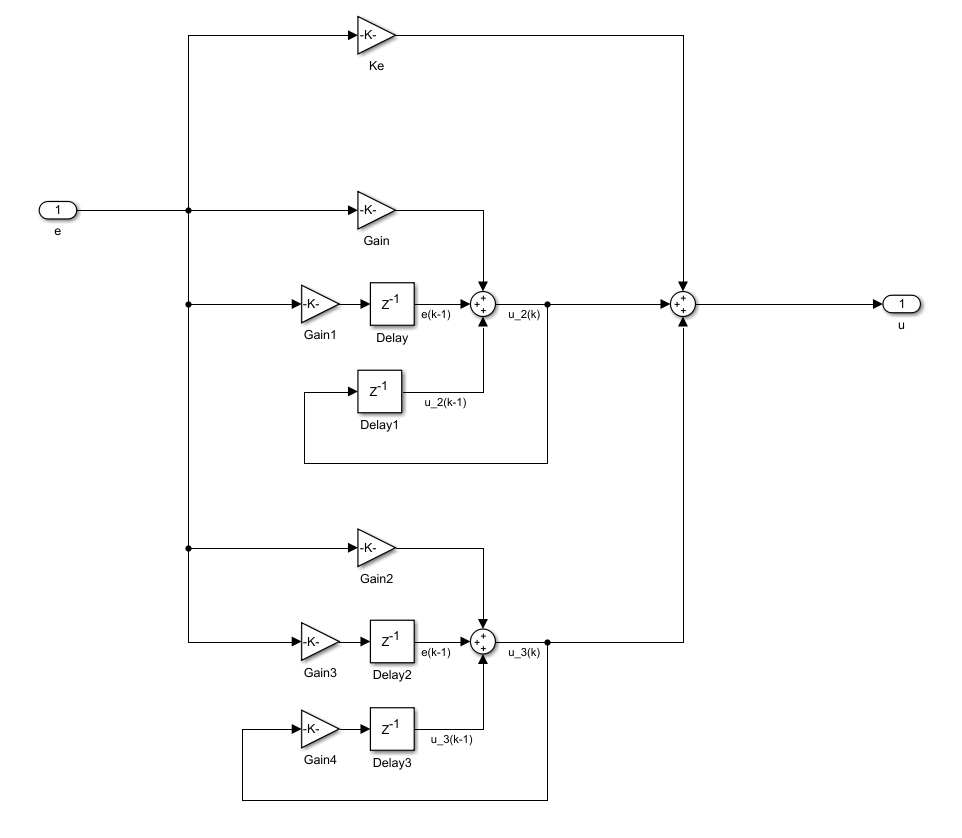
\includegraphics[width=1\textwidth]{pid_ovation_schemat.PNG}
	\caption{Schemat struktury PID (jak w systemie OVATION)}
	\label{fig::pid_ovation_schemat}
\end{figure}
\section{Realizacja regulatora PID}
Zgodnie z wytycznymi prowadzącego zaimplementowano algorytm PID taki jak w systemie OVATION. Równania opisujące algorytm:
\[
u1_k = K_e e_k
\]
\[
u2_k=u2_{k-1} + \frac{T_p}{2T_i}e_k + \frac{T_p}{2T_i}e_{k-1}
\]
\[
u2_k = \frac{2\tau_d - T_p}{T_p+2\tau_d}u3_{k-1} + \frac{2K_d}{T_p+2\tau_d}e_k -  \frac{2K_d}{T_p+2\tau_d}e_{k-1}.
\]
Parametry strojeniowe algorytmu to $K_e, T_i, K_d, \tau_d$.

Struktura w Simulinku przestawiona jest na rysunku~\ref{fig::pid_ovation_schemat}.

\section{Działanie regulatorów bez interakcji skrośnych}
Kolejnym krokiem była symulacja działania układu regulacji tylko z transmitancjami głównymi, bez transmitancji skrośnych. Do doboru nastaw wykorzystano heurystyczną metodę bazującą na wizualnej ocenie uzyskiwanych przebiegów i korekcie uzyskiwanych wartości.

W wyniku przeprowadzonych testów zdecydowano się zastosować w regulatorze wysokości regulator z członami PID, natomiast do regulacji temperatury zastosowano człony PI.

Uzyskane przebiegi na skokowe zmiany wartości zadanych przedstawiono na rysunkach~\ref{fig::pid_h_nodec_nocross} i~\ref{fig::pid_T_nodec_nocross}.
\begin{figure}[htb]
	\centering
	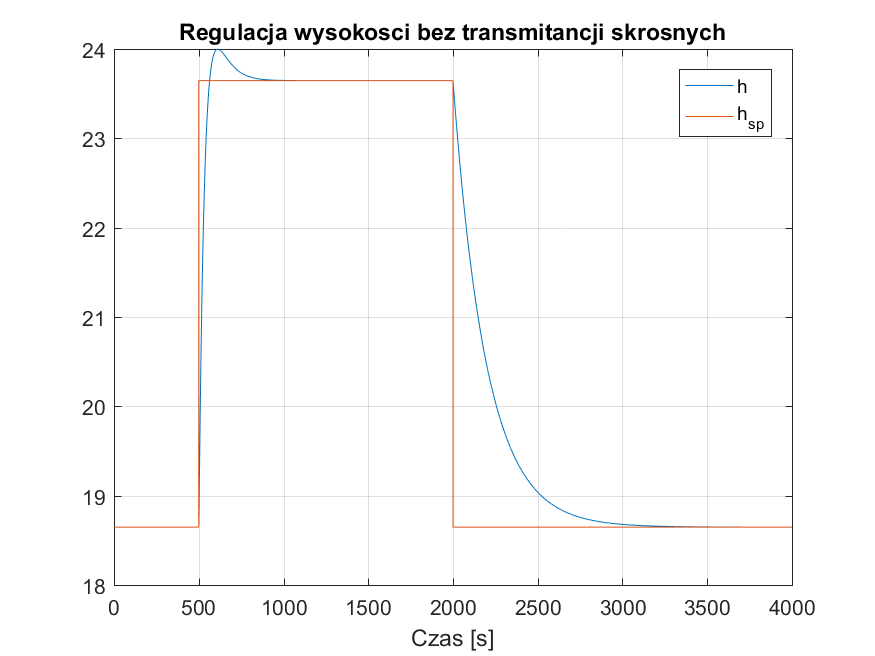
\includegraphics[width=0.85\textwidth]{pid_h_nodec_nocross.PNG}
	\caption{Działanie układu regulacji wysokości bez interakcji skrośnych. $K_e = 10, T_i = 5, K_d=4, \tau_d=2$}
	\label{fig::pid_h_nodec_nocross}
\end{figure}
\begin{figure}[htb]
	\centering
	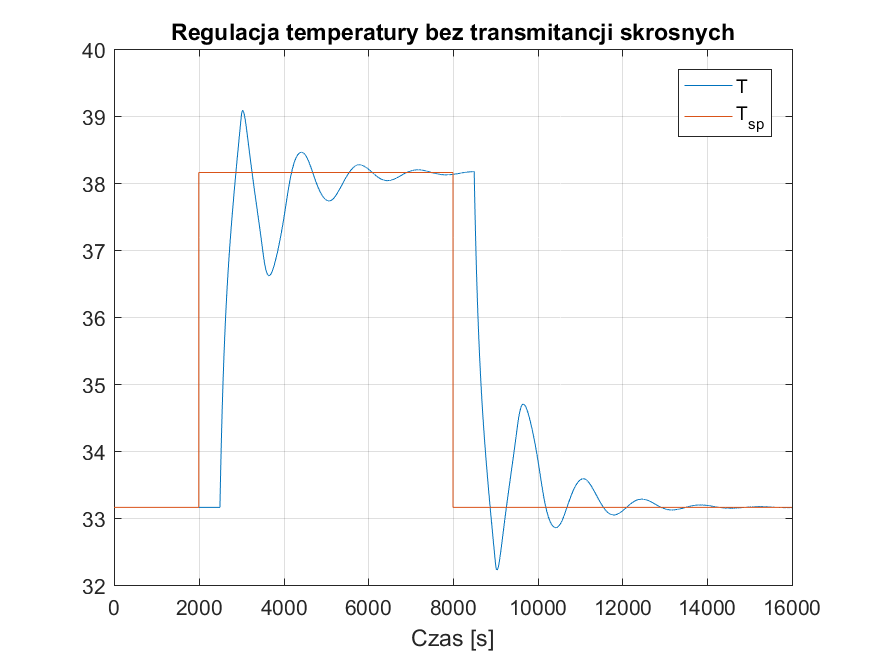
\includegraphics[width=0.85\textwidth]{pid_T_nodec_nocross.PNG}
	\caption{Działanie układu regulacji temperatury bez interakcji skrośnych. $K_e = 1.5, T_i = 350$}
	\label{fig::pid_T_nodec_nocross}
\end{figure}

Na przebiegach temperatury widoczny jest negatywny wpływ dużego opóźnienia (równego 500 sekund), czas regulacji jest dość długi. Odpowiedź układu regulacji na skok wartości zadanej cechuje się sporym przeregulowaniem, odpowiedź ma oscylacyjny charakter.

\FloatBarrier
\section{Działanie regulatorów z interakcjami skrośnymi}
Następnie uruchomiono układ regulacji z interakcjami skrośnymi, bez zmieniania nastaw uzyskanych w poprzednim punkcie. Uzyskany układ był stabilny (amplituda oscylacji malała z czasem), jednak przebiegi wartości regulowanych były dalekie od zadowalających. Przebiegi temperatury wyjściowej zawierały sinusoidę o amplitudzie kilku stopni Celsjusza, co widać na rysunku~\ref{fig::pid_hT_nodec_bad}.
\begin{figure}[htb]
	\centering
	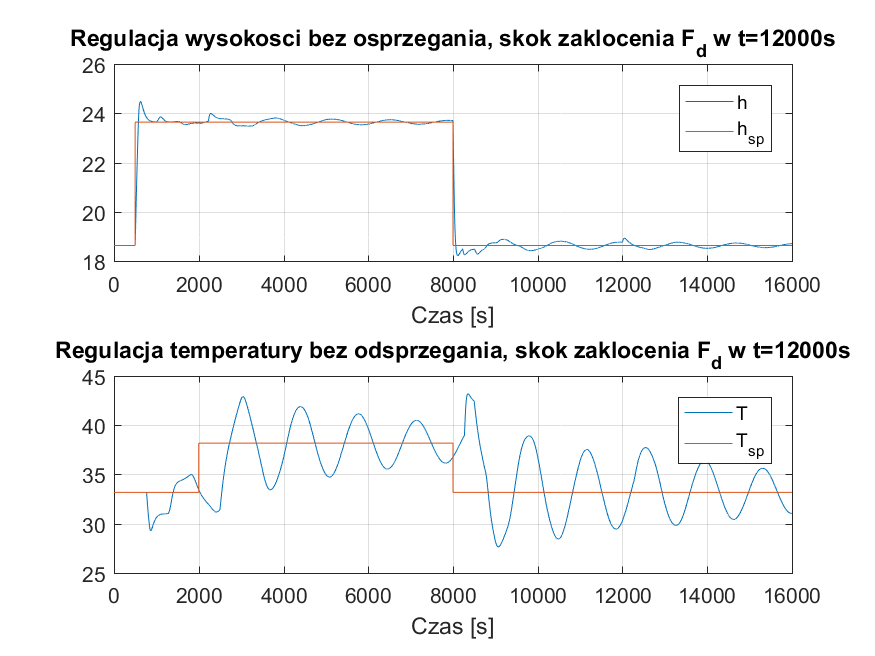
\includegraphics[width=\textwidth]{pid_hT_nodec_bad.PNG}
	\caption{Działanie układu regulacji wysokości i temperatury przy nastawach uzyskanych w poprzednim rozdziale}
	\label{fig::pid_hT_nodec_bad}
\end{figure}
\begin{figure}[htb]
	\centering
	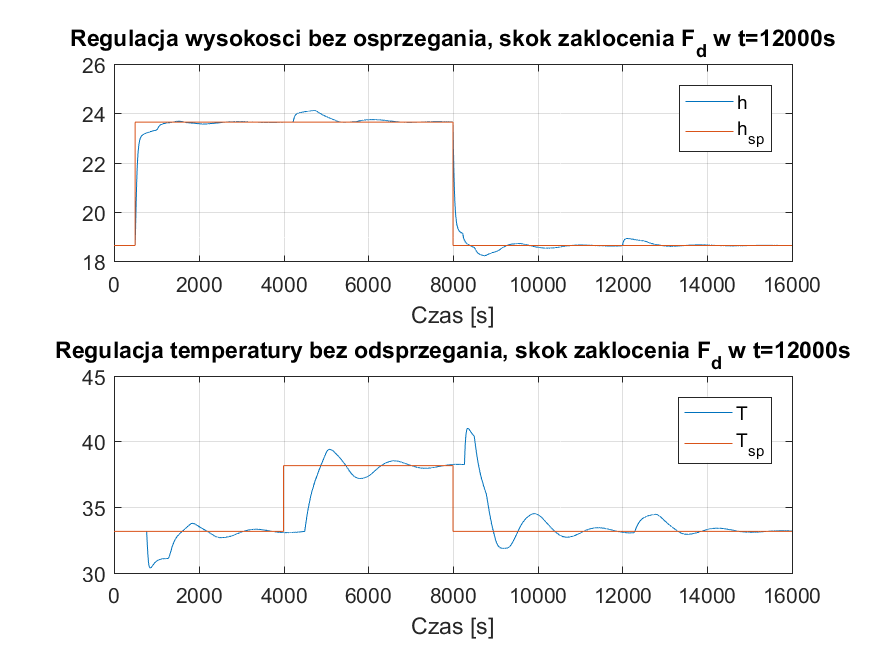
\includegraphics[width=\textwidth]{pid_hT_nodec.PNG}
	\caption{Działanie układu regulacji wysokości i temperatury. Nastawy regulatora wysokości: $K_e = 5, T_i = 50, K_d=4, \tau_d=2$, nastawy regulatora temperatury: $K_e = 1, T_i = 400$}
	\label{fig::pid_hT_nodec}
\end{figure}
Ponownie przeprowadzono dobór nastaw regulatora metodą prób i błędów. Uzyskane przebiegi wartości regulowanych (wraz ze skokiem zakłócenia $F_D$) przedstawiono na rysunku~\ref{fig::pid_hT_nodec}. Regulacja wysokości poziomu cieczy działa stosunkowo dobrze, ale regulacja temperatury jest daleka od idealnej. W przebiegach temperatury widoczne są gasnące oscylacje, czas regulacji jest długi. Niestety w analizowanym układzie (to znaczy regulatory PID i duże opóźnienia w pętli regulacji temperatury) ciężko uzyskać lepszej jakości przebiegi.

Ciekawe zachowanie układu można zaobserwować na przebiegu temperatury w okolicach czasu 8500 sekund, niedługo po skoku wartości zadanych w dół. Widoczny jest wzrost temperatury wyjściowej, podczas gdy skok zadanej temperatury był w dół. Zjawisko to jednak da się łatwo wyjaśnić. W momencie skoku wartości zadanych (czas 8000s) oba regulatory zmieniają wartość sterującą (wynikającą z obecności członu P oraz D). Regulator wysokości zmniejsza dopływ cieczy (zimnej) do zbiornika (by uzyskać spadek poziomu cieczy), a regulator temperatury zmniejsza dopływ cieczy ciepłej, by uzyskać spadek temperatury. Ze względu na obecność transmitancji skrośnych oraz fakt, że regulator wysokości może 'silniej' sterować sygnałem $F_C$ (ze względu na brak opóźnień w pętli regulacji), uzyskujemy wzrost temperatury na wyjściu. Dopiero gdy regulator temperatury 'zauważy' wzrost tej temperatury, może zareagować na tę sytuację.

\newpage
\section{Działanie regulatorów z interakcjami skrośnymi i odsprzęganiem}
\label{sec::decoupling}
W modelu uwzględniono również transmitancje osprzęgające (wyznaczone w rozdziale~\ref{sec::czlony_odsprzegajace}) $D_{12}(s)$ oraz $D_{21}(s)$, które mają postać
\[
D_{12}(s) =  -e^{-230s}
\]
\[
D_{21}(s) = 0.0776.
\]
Do obiektu wprowadzono takie same zmiany wartości zadanych oraz zakłóceń jak w poprzednim rozdziale, wynik symulacji z niezmienionymi nastawami (tzn. uzyskanymi dla układu regulacji bez odsprzęgania) przedstawiono na rysunku~\ref{fig::pid_hT_dec}.
\begin{figure}[htb]
	\centering
	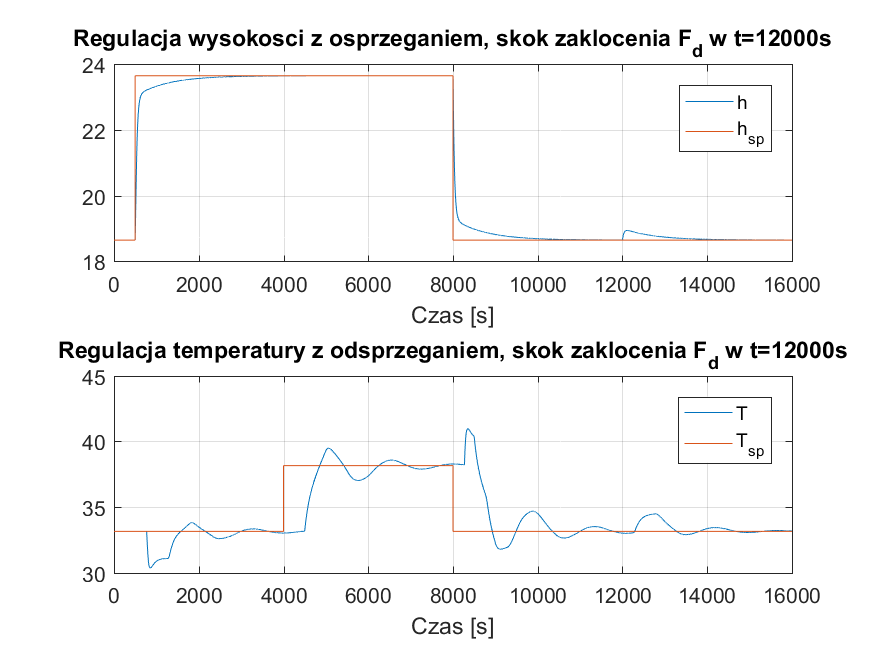
\includegraphics[width=\textwidth]{pid_hT_dec.PNG}
	\caption{Działanie układu regulacji wysokości i temperatury z odsprzęganiem. Nastawy takie jak w przebiegach na rysunku~\ref{fig::pid_hT_nodec}}
	\label{fig::pid_hT_dec}
\end{figure}

\newpage
\section{Porównanie działania układów bez i z odsprzęganiem}
Na rysunku~\ref{fig::pid_hT_comparison} przedstawiono porównanie przebiegów wartości regulowanych.

Analizując przebieg zmian wysokości poziomu cieczy nie ma wielkiego zaskoczenia, to znaczy dzięki realizowalnej postaci obliczonego członu odsprzęgającego $D_{12}(s)$ uzyskano pełne odsprzęganie, więc działanie regulatora temperatury nie 'przedostaje się' na wyjście temperatury. Uzyskane przebiegi zmian wysokości są płynniejsze. Dodanie odsprzęgania wydłuża jednak nieco czas regulacji przy skokowej zmianie zakłócenia.

W przypadku regulacji temperatury nie zaobserwowano znaczącej poprawy jakości regulacji, uzyskane przebiegi są do siebie podobne. Niestety brak możliwości zrealizowania wyliczonego członu odsprzęgającego $\widetilde{D_{21}}(s)$ sprawia, że odsprzęganie jest nieskuteczne. Opóźnienie (w zasadzie to przyspieszenie) pominięte w bloku odsprzęgającym, równe 230 sekund, jest zbyt duże względem stałej czasowej obiektu.
\begin{figure}[htb]
	\centering
	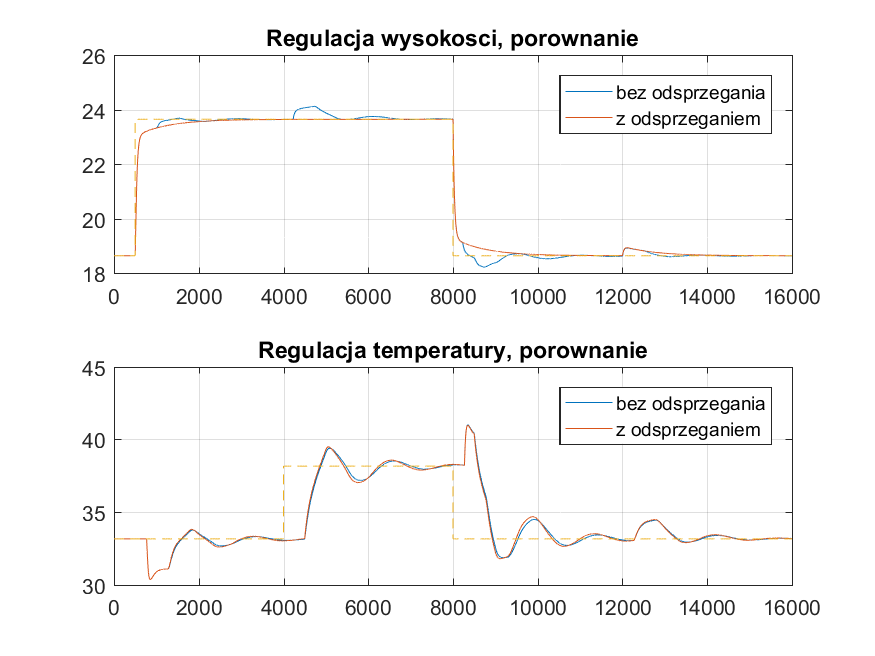
\includegraphics[width=\textwidth]{pid_hT_comparison.PNG}
	\caption{Porównanie działanie układów regulacji wysokości i temperatury bez i z odsprzęganiem}
	\label{fig::pid_hT_comparison}
\end{figure}


\section{Analiza wpływu likwidacji opóźnienia na wyjściu $T_{out}$}
W ramach dodatkowych testów przeprowadzono symulację zachowania układu w momencie, gdy nie będzie opóźnienia na wyjściu temperatury, czyli $\tau = 0s$. W takim przypadku transmitancja odsprzęgająca $\widetilde{D_{21}}(s)$ nadal ma nierealizowalne opóźnienie (przyspieszenie) i zachowanie układu jest analogiczne jak w rozdziale~\ref{sec::decoupling}. Dlatego też skupiono się na porównaniu zachowania układów bez odsprzęgania.

Pierwszym krokiem po zlikwidowaniu opóźnienia $tau$ było dostrojenie regulatora temperatury. Dzięki likwidacji sporej części opóźnienia (z 500 sekund do 230 sekund) można było nieco 'podkręcić' nastawy regulatora i uzyskać szybszą i lepszą stabilizację temperatury. Ostatecznie uzyskane nastawy regulatora temperatury to $K_e = 1.2, T_i = 350$.

Wykonano wykres porównujący zachowanie układu regulacji dla opóźnienia $tau = 270s$ oraz $tau =0s$, przedstawiono go na rysunku~\ref{fig::pid_hT_comparison_notau}.
\begin{figure}[htb]
	\centering
	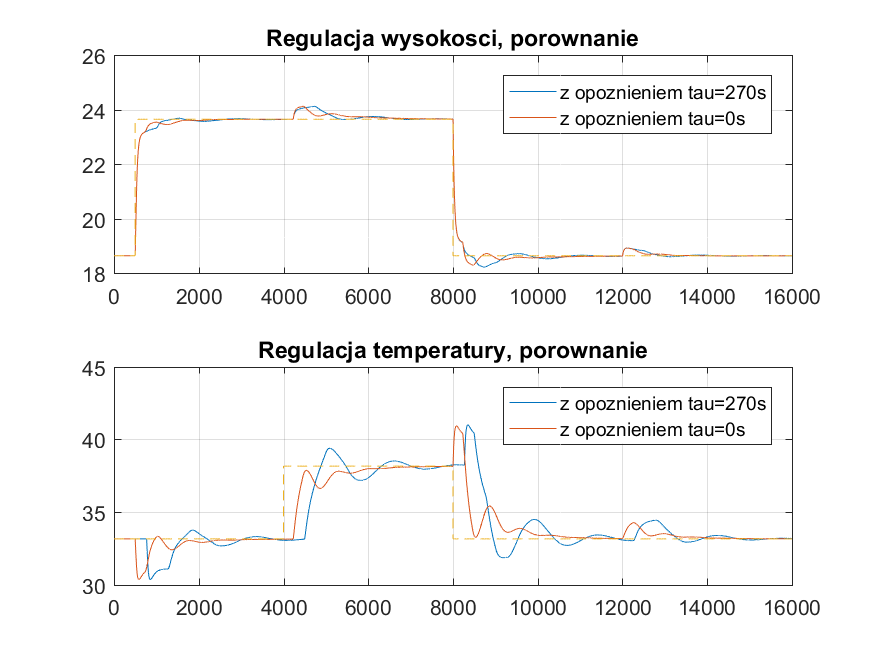
\includegraphics[width=\textwidth]{pid_hT_comparison_notau.PNG}
	\caption{Działanie układu regulacji wysokości i temperatury. Nastawy regulatora wysokości: $K_e = 5, T_i = 50, K_d=4, \tau_d=2$, nastawy regulatora temperatury: $K_e = 1.2, T_i = 350$}
	\label{fig::pid_hT_comparison_notau}
\end{figure}

Widoczna jest pozytywna zmiana w zachowaniu działania układu regulacji, szczególnie w przypadku regulacji temperatury. Układ reguluje temperaturę szybciej, a amplituda oscylacji jest mniejsza. Jest to zgodne z przewidywaniami.

Pomiar temperatury bez opóźnienia powinien być możliwy do przeprowadzenia na rzeczywistym obiekcie - wystarczy umieścić sensor temperatury na początku rury wylotowej ze zbiornika, a nie w jej dalszym biegu (zakładając, że w czasie przepływu cieczy przez rurę nie pojawiają się jakieś znaczące zakłócenia). Niewielkim kosztem można w dość znaczący sposób poprawić jakość regulacji.

\begin{thebibliography}{9}
  \bibitem{regulacja_wielopetlowa}
  Piotr Tatjewski,
  \emph{Regulacja wielopętlowa PID, wykład},
  Politechnika Warszawska,
  Warszawa, 2017.
  
\end{thebibliography}

\end{document}